\documentclass[a4paper,11pt,dvipsnames]{book}
\renewcommand{\familydefault}{\sfdefault}

\usepackage{standalone}
\usepackage[english]{babel}
\usepackage[top=3cm]{geometry}
\usepackage{float}
\usepackage{tabularx}
\usepackage{multirow}
\usepackage{booktabs}
\usepackage{pgfplots}
\usepackage{amsmath}
\usepackage{amssymb}
\usepackage{amsfonts}
\usepackage{siunitx}
\usepackage{tikz}
\usepackage{graphics} % for pdf, bitmapped graphics files
\usepackage{graphicx}
\usepackage{exsheets}
\usepackage{algorithm}
\usepackage{algorithmicx}
\usepackage[noend]{algpseudocode}
\usepackage{hyperref}
\usepackage{enumitem}
\usepackage{filecontents}
\usepackage{multirow}
%\usepackage{showframe}% to show frames
%\ifCLASSOPTIONcompsoc
\usepackage[caption=false, font=normalsize, labelfont=sf, textfont=sf]{subfig}
%\else
%\usepackage[caption=false, font=footnotesize]{subfig}
%\fi    

\usetikzlibrary{patterns,arrows,arrows.meta,calc,intersections,shapes,positioning,decorations.pathreplacing,decorations.markings,decorations.pathmorphing}
\usepackage{multicol}

\sisetup{output-decimal-marker={,},exponent-product=\cdot}

\DeclareSIUnit\atm{atm}
\DeclareSIUnit\dioptre{D}



\def\BState{\State\hskip-\ALG@thistlm}


\definecolor{TitleColor}{rgb}{0.65,0.04,0.07}
\definecolor{NumberColor}{rgb}{0.02,0.04,0.48}

\DeclareInstance{exsheets-heading}{fancy}{default}{
toc-reversed = true ,
indent-first = true ,
vscale = 2 ,
pre-code = \IfInsideQuestionT{\rule{\linewidth}{1pt}} ,
post-code =\IfInsideQuestionT{\rule{\linewidth}{1pt}} ,
subtitle-format = \large\scshape\color{rgb:red,0.65;green,0.04;blue,0.07} ,
number-format = \large\bfseries\color{rgb:red,0.02;green,0.04;blue,0.48} ,
points-format = \itshape ,
join = { number[r,B]title[l,B](.333em,0pt);
title[r,B]subtitle[l,B](1em,0pt)
} ,
attach =
{
main[hc,vc]number[hc,vc](0pt,0pt) ;
main[l,vc]subtitle[hc,vc](\marginparsep,0pt)
}
}



\DeclareInstance{exsheets-heading}{block-subtitle}{default}{
vscale = 2 ,
pre-code = \rule{\linewidth}{1pt} ,
post-code = \rule{\linewidth}{1pt} ,%title-format = \large\scshape\color{TitleColor} ,
number-format = \large\bfseries\color{rgb:red,0.02;green,0.04;blue,0.48} ,
subtitle-format = \large\scshape\color{black} ,
join = {
title[r,B]number[l,B](.333em,0pt) ;
title[r,B]subtitle[l,B](1em,0pt)
} ,
attach = {
main[l,vc]title[l,vc](0pt,0pt) ;
main[r,vc]points[l,vc](\marginparsep,0pt)
},
}

\DeclareQuestionClass{textbook}{textbooks}

\SetupExSheets{
  headings = fancy,
  question/print = true ,
  solution/print = false }
 % counter-format = se.qu ,
%  counter-within = section ,
  %question/pre-hook = \rule{\textwidth}{1pt},


\hypersetup{
	colorlinks = true, 
	breaklinks = true, 
	bookmarks = true,
	bookmarksnumbered = true,
	urlcolor = blue, 
	linkcolor = blue, 
	citecolor=blue,
	linktoc=page, 
	pdftitle={}, 
	pdfauthor={\textcopyright Author}, 
	pdfsubject={}, 
	pdfkeywords={}, 
	pdfcreator={pdfLaTeX}, % PDF Creator
	pdfproducer={IEEE} }





\tikzset{point/.style={circle,fill,black!80,inner sep=0pt,minimum size=#1,opacity=0.9}}
\tikzset{point/.default=3pt}\tikzset{vector/.style={line width=1pt,postaction={decorate,decoration={markings,mark=at position 1 with {\arrow{latex}}}}}}
\tikzset{block/.style={rectangle,fill=black!30,draw,minimum size=#1,opacity=0.9,align=center}}
\tikzset{block/.default=15pt}\tikzset{ball/.style={circle,fill=black!30,draw,minimum size=#1,opacity=0.9}}
\tikzset{ball/.default=5pt}\tikzset{pulley/.style={draw=black,line width=0.2pt,circle,minimum size=#1,inner sep=0pt,fill=black!10}}
\tikzset{pulley/.default=20pt}\tikzset{rod/.style={line width=2pt}}
\tikzset{rope/.style={line width=1pt}}
\tikzset{spring/.style={decorate,decoration={coil,amplitude=5pt,segment length=#1,aspect=0.3}}}
\tikzset{spring/.default=5pt}\tikzset{wall/.style={black!10,pattern=north east lines,opacity=0.3}}
\tikzset{ray/.style={line width=0.8pt,postaction={decorate,decoration={markings,mark=at position 0.5 with {\arrow{>}}}}}}
\tikzset{arrow/.style={-latex}}
\tikzset{object/.style={line width=1pt,orange,-latex}}
\tikzset{image/.style={line width=1pt,blue,-latex}}
\tikzset{doublearrow/.style={<->,>=latex,thick}}
\tikzset{brace/.style={decorate,decoration={brace,amplitude=#1}}}
\tikzset{brace/.default=5pt}




\graphicspath{{images/}} 




\makeatletter
\@addtoreset{question}{section}
\makeatother


\begin{document}
\author{Dr. Muhammed Rushdi \and Asem Alaa}

\title{Measurements and Instrumentation [SBE206A] (Fall 2018)\\ Tutorial 7}

\maketitle


\chapter*{Errors during the measurement process}

\section*{Introduction}
\begin{itemize}
\item Measurement errors are impossible to avoid.
\item we can minimize their magnitude by: 
\begin{itemize}
\item good measurement system design.
\item appropriate analysis and processing of measurement data.
\end{itemize} 
\item Errors are categorized to:
\begin{itemize}
\item Systematic errors
\item Random errors
\end{itemize}
\end{itemize}

\section*{Systematic errors}

The systematic errors affect the readings in a consistent way, such that all readings are on one side of the true value (either all positive or all negative).\\
\\
Sources of systematic errors are:
\begin{itemize}
\item \emph{Loading error}: system disturbances due to measurement.
\item Environmental changes (results in change of sensitivity drift or zero drift).
\item \emph{Calibration error}: use of uncalibrated instruments.
\item Wear in instruments components (can be compensated by calibration).
\item Poor cabling practices.
\end{itemize}






\section*{Random errors}

In contrast, random errors have stochastic effects on readings; the readings are distributed around a the true value.  \\ \\  
Possible sources of random errors are:
\begin{enumerate}
\item Human reading errors.
\item Electrical noise.
\end{enumerate}

\section*{Comparison between systematic and random errors}
\begin{figure*}[h!]\label{fig:uncertinity}
\centering
  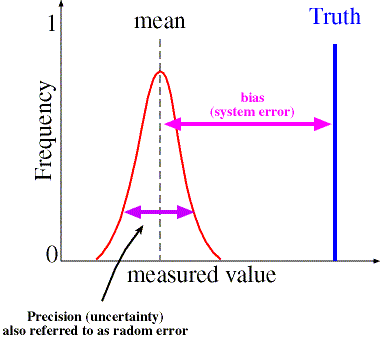
\includegraphics[width=0.8\linewidth]{uncertinity}
  \caption{Difference between systematic errors effect and random errors effect.} 
\end{figure*}

\begin{table}
\begin{tabular}{|c|c|}
\hline 
Systematic Error & Random Error \\ 
\hline 
Poor accuracy & poor precision \\ 
\hline 
definite causes & indefinite causes \\ 
\hline 
reproducible & not reproducible \\ 
\hline 
\end{tabular} 
\caption{Comparison between systematic and random errors}
\end{table}

\begin{question}
Which is more challenging? Systematic errors or random errors?
\end{question}
\begin{solution}


\end{solution}


\section*{Aggregation of measurement system errors}

\subsection*{The worst-case prediction of maximum error}

\begin{equation}
\text{error} = \sum_{i}^{n} x_i
\end{equation}

\subsection*{Likely maximum systematic error}

\begin{equation}
\text{error} = \sqrt{ x_{1}^{2} + x_{2}^{2} + \ldots + x_{n}^{2} }
\end{equation}

\chapter*{Problems}

\section*{Systematic Errors}
\subsection*{Systematic erros due to disturbance}
\begin{question}[subtitle=System Disturbance]
\begin{figure*}[h!]\label{fig:systematic_error_circuit}
\centering
  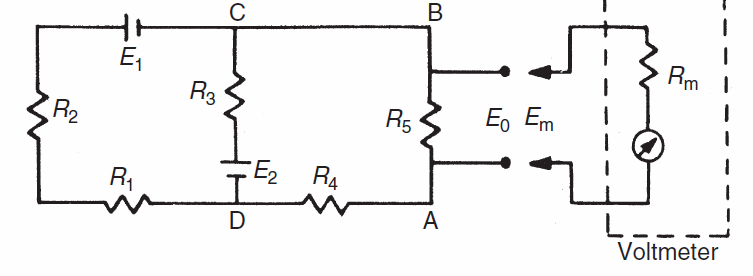
\includegraphics[width=0.8\linewidth]{systematic_error_circuit}
  \caption{Effect of applying the voltmeter to the measured quantity.} 
\end{figure*}
\begin{enumerate}
\item Derive the relation of the true and output readings.
\item Suppose that the components of the circuit in Figure \ref{fig:systematic_error_circuit} have the following values:
 R\textsubscript{1} = $400\Omega$, R\textsubscript{2} = $600\Omega$, R\textsubscript{3} = $1000\Omega$, R\textsubscript{4} = $500\Omega$, R\textsubscript{5} = $1000\Omega$
\end{enumerate}
\examspace*{15em}

\end{question}
\begin{solution}


\end{solution}


\begin{question}
An inexpensive voltmeter is used to measure the voltage to with 1 \%
across the power terminals of a stereo system. Such a system typically has
an output impedance of 500 $\Omega$ and a voltage of 120 V at its power terminals.
Assuming that the voltmeter is 100 \% accurate such that the instrument and
zero-order uncertainties are negligible, determine the minimum input impedance
(in $\Omega$) that this voltmeter must have to meet the 1 \% criterion.

\examspace*{15em}

\end{question}
\begin{solution}


\end{solution}


\begin{question}\label{problems:1}

\begin{figure*}[h!]\label{fig:problem}
\centering
  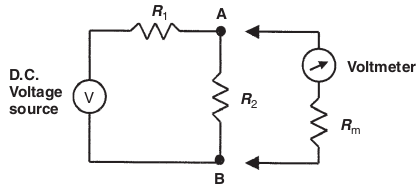
\includegraphics[width=0.8\linewidth]{problem}
  \caption{Circuit for Exercise ~\ref{problems:1}} 
\end{figure*}

In the circuit shown in Figure \ref{fig:problem}, the resistor values are given by $\rm R_1 = 1000 \Omega$; $ \rm R_2 = 1000 \Omega$; V = 20 volts. The voltage across AB (i.e., across $\rm R_2$ ) is measured by a
voltmeter whose internal resistance is given by $\rm R_m = 9500 \Omega$.
\begin{enumerate}
\item What will be the reading on the voltmeter?
\item What would the voltage across AB be if the voltmeter was not loading the circuit (i.e., if $\rm R_m = \infty $)?
\item show that the voltage $\rm E_m$ measured across points AB by the voltmeter is related to the true voltage ($\rm E_o$) by the following expression:
\begin{equation}
\rm \frac{E_m}{E_o} = \frac{R_m( R_1 + R_2 )}{R_1(R_2+R_m)+R_2 R_m}
\end{equation}
\item What is the measurement error due to the loading effect of the voltmeter?
\item If the parameters in Figure \ref{fig:problem} have the following values, $\rm R_1 = 5000 \Omega$; $\rm R_2 = 10000 \Omega$; what value would the voltmeter internal resistance $\rm R_m$ need to be in order not to exceed a measurement error of 1\%?
\end{enumerate}
\examspace*{20em}

\end{question}
\begin{solution}


\end{solution}

\begin{question}\label{problems:2}

\begin{figure*}[h!]\label{fig:problem2}
\centering
  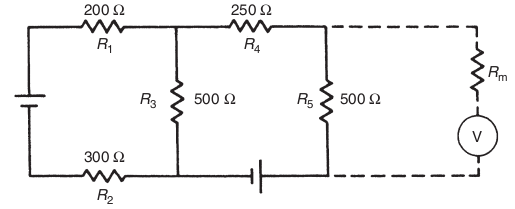
\includegraphics[width=0.8\linewidth]{problem2}
  \caption{Circuit for Exercise ~\ref{problems:2}} 
\end{figure*}

The voltage across a resistance $\rm R_5$ in the circuit of Figure \ref{fig:problem2} is to be measured by a voltmeter connected across it.
\begin{enumerate}
\item If the voltmeter has an internal resistance ($\rm R_m$) of $4750 \Omega$, what is the measurement error?
\item What value would the voltmeter internal resistance need to be in order to reduce the measurement error to 1\%?
\end{enumerate}

\examspace*{15em}

\end{question}
\begin{solution}


\end{solution}


\begin{question}

A requirement for a resistance of $1220 \Omega$ in a circuit is satisfied by connecting together resistances of 1000 and 220 $\Omega$ in series. If each resistance has a tolerance of $\pm 5\%$, what is the likely tolerance in the total resistance?
\examspace*{10em}

\end{question}
\begin{solution}


\end{solution}

\begin{question}
In order to calculate the heat loss through the wall of a building, it is necessary to know the temperature difference between inside and outside walls. Temperatures of 5 and 20 $^{\circ}$C are measured on each side of the wall by mercury-in-glass thermometers with a range of 0 to $\rm \pm 50^{\circ}C$ and a quoted inaccuracy of $\pm 1\%$ of full-scale reading.
\begin{enumerate}
\item Calculate the likely maximum possible error in the calculated value for the temperature difference.
\item Discuss briefly how using measuring instruments with a different measurement range may improve measurement accuracy.
\end{enumerate}
\examspace*{10em}

\end{question}
\begin{solution}


\end{solution}
\end{document}